% Conduct a comprehensive review of the existing literature 
% on artificial intelligence and machine learning techniques 
% used in weather prediction. Discuss the strengths and limitations 
% of these approaches

% The literature review section of your thesis is a critical component 
% of your research, as it provides a comprehensive overview of the 
% current state of knowledge on the topic of weather prediction and 
% the application of artificial intelligence and machine learning 
% techniques in this area. Here are some important elements to consider 
% including in your literature review:

% Overall, your literature review should provide a comprehensive overview of 
% the existing literature on weather prediction and the application of artificial 
% intelligence and machine learning techniques in this area. It should also 
% highlight the importance of your research question, and explain how your research 
% contributes to the broader understanding of the field.
\section{Przegląd literatury}

Jako już dojrzała metodologia, zastosowanie uczenia maszynowego 
znajduje dużą duże odbicie w wielu artykułach i publikacjach naukowych. 
Wiele publikacji analizuje zastosowanie AI w hybrydowych, jak i czystych 
algorytmach prognozowania pogody. 


% Background information: Begin by providing some background information on 
% the topic of weather prediction and the challenges that exist in this area. 
% This could include discussing the impact of weather on human life and the 
% economy, the limitations of current weather prediction methods, and the potential 
% benefits of using artificial intelligence and machine learning techniques to 
% improve accuracy.
\subsection{Tło teoretyczne}


\subsubsection{Metody NWP}

Pierwsze próby "odręcznych" modeli NWP były zainicjowane przez Lewis Fry Richardson-a w 1922 roku i 
były zainspirowane ideą przewidywania pogody za pomocą sformułowanych praw fizyki. Sformułowanie
nieliniowych równań różniczkowych opisujących pogodę tworzyło problem z wartością początkową bazującą
na bieżących pomiarach pogody. W celu osiągnięcia zamierzonego celu interakcje z dziedziny 
termodynamiki, dynamiki, procesów chemicznych, jak i biologicznych muszą być wzięte pod uwagę.
Pierwsze komputerowo wspomagane prognozy pogody były tworzone już w 1950 roku, lecz dopiero
w 1970 roku wraz z rozwojem superkomputerów rozwiązanie pełnego zbioru równań było możliwe.

Podstawowymi równaniami opisującymi zachowanie pogody są równania Naviera-Stokesa, równania zachowania
masy, pierwsza zasada termodynamiki i równanie Clapeyrona. Za pomocą nich stan wiatru, ciśnienia,
gęstości, temperatury może być modelowany opisując stan atmosfery. Ze względu na brak rozwiązania
analitycznego tych równań, koniecznością jest rozwiązanie numeryczne. Procesy fizyczne występujące
w zbyt małej skali, aby być ujęte podczas dyskretyzacji przestrzeni, muszą być opisywane za pomocą
parametryzacji próbujących przybliżyć ich wpływ na ogólne rozwiązanie. W wielu przypadkach 
dodatkowe uproszczenia i zaokrąglenia są brane pod uwagę w celu uproszczenia procesu
rozwiązywania. Niektóre modele globalne i prawie wszystkie modele lokalne stosują 
metodę różnic skończonych we wszystkich stopniach swobody systemu, a niektóre modele globalne
wykorzystują metodę różnic skończonych w kierunku pionowym a metody spektralne w kierunku równoległym
do powierzchni ziemi. Krok czasu stosowany w stosunku do modeli globalnych jest wielkości dziesiątek
minut, a w przypadku prognoz lokalnych w zakresie jednej do czterech minut.

\begin{figure}[H]
    \centering
    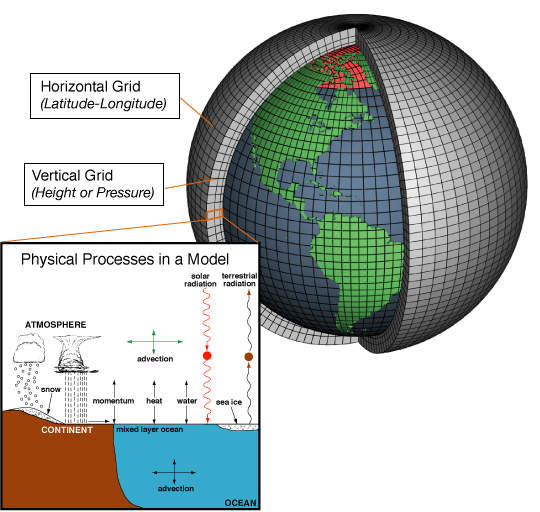
\includegraphics[width=\textwidth]{images/grid.png}
    \caption[opis dla siatki]{Obraz pokazujący sposób dyskretyzacji przestrzeni
    na siatkę parametrów\footnotemark}
    \label{grid}
\end{figure}

\footnotetext{Źródło: \url{https://en.wikipedia.org/wiki/File:AtmosphericModelSchematic.png}}

Ze względu na chaotyczną charakterystykę równań opisujących pogodę, małe zmiany w warunkach początkowych
mogą skutkować odstającymi od siebie wynikami. W celu opisania i przewidywania błędu prognozy pogody 
rozwinięte zostały modele ensemble. Nieliniowa złożoność systemu oznacza, że podejścia opisu
dokładności prognozy bazujące na metodach czysto statystycznych nie przynoszą upragnionych wyników.
Dlatego zbiór wielu modeli zainicjowanych z nieznacznie różniącymi się warunkami początkowymi
jest stosowany do sprawdzenia jak bardzo uzyskane wyniki mogą się różnić, i nadania dokładności do 
stworzonej prognozy. Przykładowa predykcja stworzona przy pomocy metody ensemble znajduje się 
poniżej\ref{nwp-ensemble}.

\begin{figure}[H]
    \centering
    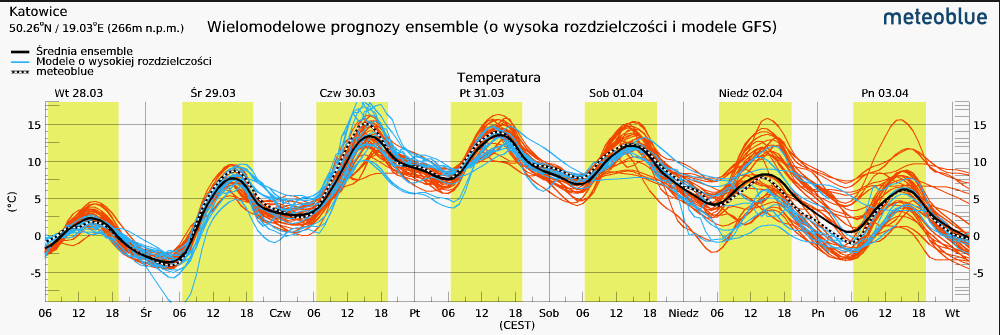
\includegraphics[width=\textwidth]{images/multimodel.png}
    \caption[ensemble]{Przykładowy wynik działania modelu ensemble\footnotemark}
    \label{nwp-ensemble}
\end{figure}
\footnotetext{Źródło: \url{https://www.meteoblue.com/pl/pogoda/prognoza/multimodel/katowice_polska_3096472}}

Wczesne metody specyfikacji warunków początkowych opierały się na analizie graficznych wykresów 
pogodowych. Następnie różne metody interpolacji danych były zastąpione przez algorytmy
asymilacji danych oparte na teorii sterowania optymalnego. Obliczanie rzeczywistych wartości
opisujących atmosferę może być opisane jako wnioskowane Bayesowskie oparte na wynikach pomiarów
oraz ich niepewnościach. Te obliczenia skoncentrowane na minimalizacji obiektywnej funkcji 
są przeprowadzane w czterowymiarowej przestrzeni, aby otrzymać fizycznie możliwy wynik
równomiernie rozłożony w trzech wymiarach przestrzennych i czasie.

W praktyce wykorzystanie modeli NWP w celach predykcji pogody wymaga asymilacji dużej ilości
danych pochodzących z różnych źródeł. Metodą wykorzystywaną dzisiaj w celu wprowadzenia
danych jest asymilacja 4D-Var (używana od 1980 roku). W tym algorytmie dla każdego typu obserwacji tworzony jest
operator obserwacji pozwalający wewnętrznym parametrom modelu NWP na odniesienie się
do poszczególnego typu obserwacji. Podczas procesu asymilacji danych parametry wewnętrzne
modelu są dostosowywane, aby jak najlepiej odzwierciedlić rzeczywiste warunki pogodowe.

W wielu przypadkach złożoność obliczeniowa NWP wymaga redukcji objętości danych pochodzących
z obserwacji satelitarnych o dużej gęstości. Rozdzielczość danych pochodzących z odczytów
satelitarnych znacznie przekracza możliwości dotychczas używanych modeli stworzonych przez
ECMWF posiadających rozdzielczość horyzontalną równą 9 km. Co więcej, w przypadku modeli
ensemble w celach zmniejszenia kosztów obliczeniowych rozdzielczość jest zmniejszana do 18 km.
Procesy, które nie mogą być wiernie odzwierciedlone przez symulację
ze względu na zbyt małą rozdzielczość NWP podlegają parametryzacji.
Do takich procesów zalicza się: formowanie się chmur, ilość promieni słonecznych docierających do 
podłoża, opór aerodynamiczny szczytów górskich czy formowanie się kropelek wody.

Ostateczny wynik przeprowadzonej symulacji NWP musi być jeszcze dodatkowo wzbogacony przez zastosowanie
statystyk wyjścia modelu (MOS). W ramach tego prognozowany stan modelu opisywany poprzez skomplikowane
parametry jest zamieniany na wielkości łatwo interpretowane przez ludzi. Co więcej, metody numeryczne
wykorzystują przybliżoną siatkę modelującą atmosferę, która musi być interpolowana w celu uzyskania
wyniku dla konkretnej lokalizacji. W tych celach często stosuje się wielokrotne zastosowanie 
regresji liniowej. Krok ten dodatkowo umożliwia zniwelowanie błędów nawarstwionych przez model i wzięcie
pod uwagę sparametryzowanych zjawisk.

Dodatkowo niektóre parametryzacje także są stopniowo zastępowane przez algorytmy uczenia maszynowego,
czego przykładem jest obliczanie energii promieniowania w sposób uproszczony
\cite{ai-in-weather-and-climate-prediction}. Energia promieniowania
może być w sposób kosztowny obliczona przez modele NWP, lecz zastosowanie ML skutkuje szybszym
procesem prognozowania.

Przykładowymi modelami prognozowania pogody są Lorenz63 i Lorenz96\cite{ai-in-weather-and-climate-prediction}
które są najprostsze w opisie,
które są zaprojektowane z mniejszą ilością stopni swobody. Modele te są łatwe w zrozumieniu i 
stanowią podstawe do przeprowadzania badań. Ich szybka natura sprawia, że ich stosowanie jest dość
proste, niestety dokładność predykcji jest dość niska. Przeciwieństwem do nich są modele NWP i GCM,
które są bardzo skomplikowane i trudne do zrozumienia, są opisane przez wielowymiarowe równania, oraz
osiągają większą dokładność.

\begin{figure}[H]
    \centering
    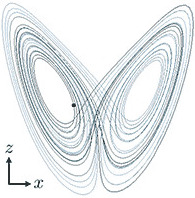
\includegraphics[width=0.5\textwidth]{images/lorenz.jpeg}
    \caption[lorenz]{Wykres pokazujący atraktor lorenza - matematyczny opis chaotycznej 
    charakterystyki równań różniczkowych wynikających z analizy pogody.\footnotemark}
    \label{lorenz}
\end{figure}
\footnotetext{Źródło: \url{https://en.wikipedia.org/wiki/File:A_Trajectory_Through_Phase_Space_in_a_Lorenz_Attractor.gif}}

Jednym z większych problemów NWP jest nieliniowo wzrastający błąd ograniczający długość prognozy.
Ponieważ modele NWP dokonują predykcji w sposób stopniowy, prognozując stan systemu dla następnego
kroku, żeby później otrzymany wynik dodać do danych wejściowych i kontynuować obliczenia, otrzymane błędy
mają tendencję do akumulacji wraz ze wzrostem długości symulacji.
Limit dla wydarzeń o małej skali jest szacowany na dni bądź godziny, zdarzenia o dużej skali
mogą być prognozowane z aż 2 tygodniowym wyprzedzeniem. Szacuje się, że błąd akumulowany przez 
model NWP ulega zdwukrotnieniu z każdymi pięcioma dniami.

W porównaniu z wieloma innymi dziedzinami, w których numeryczne prognozowanie jest stosowane,
NWP ma przewagę pod względem częstotliwości, z którą jest wykorzystywane. Prognozy są generowane
w ten sposób z częstotliwością dzienną i na poziomie globalnym. Dokładność tworzonych predykcji jest
dobrze znana i sposoby wzmocnienia aktualnie stosowanych algorytmów mogą być sprawdzone z dużą
efektywnością. Modele NWP wciąż są ulepszane, a rozwój technologiczny i naukowy być może pozwoli
w przyszłości tworzyć modele bazujące na danych zbieranych z rozdzielczością sięgającą 1 km. Co więcej,
możliwe że w najbliższej przyszłości utworzone zostaną modele rozwiązujące sprzężone symulacje
dla atmosfery, lądu oraz oceanu\cite{nwp-the-quiet-revolution}.

Dzisiejsze komputery używane do NWP sięgają mocy obliczeniowej równej jednego petaflop-a ($10^{15}$ operacji
zmiennoprzecinkowych) na sekundę. Szacuje się, że systemy komputerowe stosowane przez ECMWF mają zużycie energii
sięgające 10 MVA, a dalszy rozwój i zwiększenie modeli mogłoby wymagać 10-krotne zwiększenie pobieranej mocy.

\subsubsection*{Metody uczenia maszynowego}

Problem prognozowania pogody można opisać przy pomocy metody regresji. Polega ona
na statystycznym modelowaniu odpowiedzi nieznanych wartości funkcji na podstawie
znanych wartości zmiennych niezależnych. W ramach przewidywania pogody, za zmienne niezależne
można przyjąć znane wartości pomiarów atmosferycznych i przy pomocy regresji oszacować 
wartości przewidywane. Użyteczne mogą być także metody klasyfikacji w celu wykrywania i 
przewidywania zjawisk pogodowych. W następującej pracy jednak w celu prognozowania pogody
zastosowane będą następujące metody regresji z zakresu uczenia maszynowego:


\begin{itemize}
    \item SVR — jest metodą regresji wykorzystującą maszynę wektorów nośnych w celu tworzenia
    predykcji. Opiera się ona na tworzeniu hiperpłaszczyzny mającej na celu z jak największą
    dokładnością rozdzielenie obserwacji ze zbioru treningowego. Następnie wyznaczone
    równanie hiperpłaszczyzny jest wykorzystywane do klasyfikacji i liczenia regresji dla naukowych
    danych.

    Obliczenie równania hiperpłaszczyzny sprowadza się do problemu optymalizacyjnego
    maksymalizowania odległości hiperpłaszczyzny od punktów należących do poszczególnych klas.
    Ponad przeprowadzanie regresji liniowej, SVR jest w stanie tworzyć regresji nieliniowe
    poprzez zastosowanie "kernel trick", niejawnie mapując dziedzinę danych wejściowych na 
    wielowymiarową przestrzeń o innej charakterystyce.
    
    \item Regresja Logistyczna — jest modelem statystycznym przewidującym nastąpienie danego
    zdarzenia na podstawie obliczenia funkcji logitowej z kombinacji liniowej zmiennych 
    niezależnych.

    \item SGD — jest metodą trenowania modeli uczenia maszynowego poprzez iteratywną optymalizację
    funkcji celu. Zastosowanie SGD uzyskało dobre wyniki w trenowaniu modeli stosowanych
    do klasyfikacji tekstu i przetwarzaniu języka naturalnego. W ramach tego algorytmu
    punkt początkowy wybierany przez użytkownika jest poddawany iteratywnej optymalizacji
    poprzez wybieranie kierunku największego spadku funkcji błędu. W ten sposób przestrzeń rozwiązań
    jest przeszukiwana w bardzo efektywny sposób. Niestety zapewnienie globalnego minimum
    nie jest zawsze zagwarantowane.

    \item KNN — jest prostym modelem, który może być stosowany zarówno do regresji, jak i klasyfikacji.
    Polega na wybraniu k najbliższych sąsiadów ze zbioru treningowego, aby określić wartość dla nowej
    obserwacji. Po wybraniu najbardziej podobnych obserwacji ze zbioru treningowego wartość funkcji
    celu jest uśredniana.

    \item Regresja Gaussowska — jest nieparametryczną formą metody Bayesowskiej do tworzenia
    predykcji. Zamiast obliczać dystrybucję parametrów funkcji ta metoda może być zastosowana do
    obliczenia dystrybucji funkcji celu.
    
    \item PLS — Partial least squares regression- jest algorytmem wykorzystującym rozkład
    danych ze względu na analizie głównych składowych (PCA), aby w następnym wykorzystać metodę
    najmniejszych kwadratów do przeprowadzenia regresji.

    \item Drzewo Decyzyjne — jest modelem o strukturze drzewiastej, której celem jest
    przewidzenie wartości funkcji celu na podstawie podzbioru wartości atrybutów obserwacji. 
    Drzewa decyzyjne są budowane na podstawie rekursywnego partycjonowania danych treningowych
    ze względu na atrybut optymalizujący miarę dopasowania drzewa (Gini, zysk informacyjny).
    Ze względu na różne użyte miary i metody budowania drzewa wyróżnia się algorytmy ID, C4.5,
    C5.0 oraz CART. W użytej bibliotece sklearn zaimplementowany i użyty jest ten ostatni.

    \item Las Losowy — algorytm, w którym tworzona jest duża liczba drzew decyzyjnych poprzez
    bootstraping i bagging oryginalnego zbioru danych. Ostateczna decyzja lasu losowego w 
    zadaniu regresji jest średnią z wyjścia wszystkich wygenerowanych drzew decyzyjnych.

    \item MLP — perceptron wielowarstwowy. Najprostszy typ sieci neuronowej. Składa się z 
    warstwy wejściowej, warstw ukrytych oraz warstwy wyjściowej. Każda warstwa składa się
    z pewnej liczby perceptronów mających naśladować działanie neuronów w ludzkim mózgu.
    Wartość wyjściowa każdego perceptrona jest obliczana jako wartość funkcji aktywacji z 
    liniowej kombinacji wartości na wejściu. Każda kolejna warstwa sieci jest gęsto połączona
    z warstwą poprzednią.
    Proces uczenia sieci neuronowej polega na zastosowaniu propagacji wstecznej, aby dostosować
    wartości parametrów sieci, w celu minimalizacji funkcji błędu określającej jak daleko
    wyjście sieci odbiega od pożądanej wartości. 

    \item RNN — są klasą sieci neuronowych, w których połączenia pomiędzy węzłami
    mogą tworzyć cykle, pozwalając na to, aby wyjście z niektórych węzłów mogło mieć wpływ na 
    wejście tych samych węzłów. Ta charakterystyka sieci pozwala na objaśnienia tymczasowych 
    zachowań dynamicznych. Wewnętrzny stan sieci rekurencyjnych (pamięć) może być wykorzystywany
    do przetwarzania danych o zmiennej długości. Znajdują szerokie zastosowanie w rozpoznawaniu
    pisma lub mowy. Przykładowymi warstwami charakteryzującymi sieci rekurencyjne są LSTM bądź GRU.
    Sieci te zostały specjalne zaprojektowane do celów analizy danych o czasowo zależnej naturze.

    \item CNN — są klasą sieci neuronowych, w której wykorzystywane są konwolucje w celu 
    analizy i preprocesowania danych wejściowych. Pozwalają na przetwarzanie danych wielowymiarowych
    w ustrukturyzowany sposób. Są często wykorzystywane w celu klasyfikacji obrazów, wideo czy
    audio. Mogą być jednak używane w stosunku do każdych danych wykazujących zorganizowaną strukturę.

\end{itemize}

% Overview of existing literature: Provide a comprehensive overview of the 
% existing literature on weather prediction and the use of artificial intelligence 
% and machine learning techniques in this area. This could involve summarizing the 
% findings of previous studies, identifying key themes and trends, and highlighting 
% any gaps or limitations in the current literature.
\subsection{Istniejące źródła}

Można znaleźć artykuły analizujące najczęściej występujące słowa
w publikacjach dotyczących algorytmów przewidywania pogody 
\cite{ml-in-weather-prediction}. Okazuje się, że w artykułach traktujących o
metodach NWP najczęściej występującą frazą jest "prognozowanie wiatru". Innymi 
często występującymi sformułowaniami były "modele ensemble", "asymilacja danych",
"warunki ekstremalne". Pośród analizowanych artykułów słowo wiatr pojawiło się
ponad 200 razy, najczęściej w odniesieniu do źródeł odnawialnej energii i badań
w przewidywaniu siły wiatru. Słowo opady pojawiło się prawie 150 razy, zazwyczaj
odnosząc się do wykorzystania w prognozowaniu krótkoterminowym, post-processingu, czy
downscaling. 

Z kolei dla artykułów dotyczących uczenia maszynowego
w dziedzinie klimatu najczęściej występujące frazy to "zmiana klimatu", 
"wpływ na klimat", "warunki ekstremalne". Okazuje się, że o wiele częstsze było
wystąpienie określenia "globalne modele klimatyczne" niż "regionalne modele 
klimatyczne". 

Wśród istniejących publikacji popularnymi tematami są także korekcja odchylenia 
temperatury i ciśnienia atmosferycznego, analiza promieniowania słonecznego w celach
zasilania instalacji fotowoltaicznych.

\subsubsection*{Wyniki analizowanych źródeł}

\Citeauthor*{machine-learning-for-applied-weather-prediction}
\cite{machine-learning-for-applied-weather-prediction} stworzyli system 
o nazwie DICast podnoszący dokładność modeli numerycznych o 10-15\% przy pomocy
uczenia maszynowego. Zaletą zastosowanego przez nich podejścia jest możliwość
użycia małego zbioru danych do treningu oraz dynamicznej aktualizacji do 
najnowszych informacji.

Badania podsumowane w  przez  \Citeauthor*{ai-revolutionises-weather-prediction}
\cite{ai-revolutionises-weather-prediction}
stwierdzają polepszenie dokładności metod numerycznych ulepszonych przy
pomocy ML w stosunku do bazowych modeli. Odnotowane polepszenie wyników
sięgało 12.4\% dla wilgotności, 5.2\% dla prędkości wiatru, 17.0\% dla
temperatury.

\Citeauthor*{weather-monitoring-using-artificial-intelligence}\cite{weather-monitoring-using-artificial-intelligence}
wybrali regresję liniową do modelowania pogody i zaobserwowali 3.5-procentową
dewiację dla prognozy na następny dzień.

Porównanie wielu modelów, w tym sieci neuronowej, sieci radialnej, 
drzew GBT, regresji liniowej i lasu losowego przez 
\Citeauthor*{developing-machine-learning-algorithms}
\cite{developing-machine-learning-algorithms} wskazuje na 
najlepsze wyniki uzyskiwane przez sieć neuronową. Osiągnęła ona 
współczynnik korelacji równy 84.62\% w zadaniu prognozowania
pogody z miesięcznym wyprzedzeniem. Także \Citeauthor*{weather-forecasting-using-dl} 
\cite{weather-forecasting-using-dl} wskazuje na dobrą dokładność
sieci neuronowych podczas prognozowania opadów.

\Citeauthor*{ml-applied-to-weather-forecasting}
\cite{ml-applied-to-weather-forecasting} wnioskuje że metody 
numeryczne są w stanie osiągnąć lepsze wyniki dla prognoz 
krótkoterminowych, lecz różnica dla prognoz długoterminowych
nie była już tak znaczna. Proponowanym wytłumaczeniem tego jest
brak stabilności modeli NWP i akumulacja błędów dla dłuższych 
okresów. Z kolei uczenie maszynowe zdaje się bardziej
odporne na perturbacje w warunkach początkowych i zachowuje 
stabilne wyniki nawet dla prognoz długoterminowych.

Mimo wszystko kwestia zastąpienia NWP przez metody uczenia maszynowego
wciąż nie jest rozstrzygnięta jak wskazuje \Citeauthor*{can-dl-beat-numerical}
\cite{can-dl-beat-numerical}. Artykuł ten szacuje jakość prognoz 
deterministycznych publikowanych przez ECMWF na 80\% dokładności w przewidywaniu
poziomu ciśnienia na przełomie 7 dni. Z kolei temperatura może być 
prognozowana z błędem średnio-kwadratowym równym 2 stopnie. Wśród wymienionych
zastosowań uczenia głębokiego było szacowanie dystrybucji parametrów przy pomocy 
sieci rekurencyjnej i konwolucyjnej. Innym zastosowaniem było uchwycenie
niepewności z obserwacji w kontekście prognozowania opadów.

Jednym z bardziej wszechstronnych źródeł porównujących aż 24 modele z zakresu
uczenia maszynowego był \Citeauthor*{comparison-of-ml-methods}\cite{comparison-of-ml-methods}.
W tej pracy autor porównywał wybrane modele w celu przewidywania energii fotowoltaicznej
na następny dzień bazując na algorytmach NWP. W tym celu zastosowane było pięć metryk
weryfikacyjnych. Najlepszym modelem w przedstawionym problemie okazała się regresja 
kernel-ridge, wykazująca się także najdłuższym czasem treningu i wysokim zużyciem pamięci.
Algorytmem zalecanym do wykorzystania praktycznego był perceptron wielowarstwowy (MLP)
osiągający zbliżone wyniki do regresji kernel-ridge, lecz wymagający o wiele mniej zasobów.
Co więcej, jednym z wniosków tej pracy jest duże znaczenie wyboru zmiennych w danych wejściowych
na jakość wytrenowanego modelu. Powiększenie danych o dodatkowe informacje przyniosło
wyniki lepsze o 13.1\% w porównaniu do podstawowych zestawów atrybutów. Dalsze polepszenie
mogło być uzyskane poprzez dostrojenie hiperparametrów, umożliwiające zmniejszenie 
RMSE o 3.1\%. Dostosowanie hiperparametrów miało większy wpływ w algorytmach opartych
na drzewach decyzyjnych niż MLP, gradient boosting czy regresji. 

Kolejnym artykułem z tej dziedziny jest \Citeauthor*{coupling-data-science}\cite{coupling-data-science}
analizujący wartość nasłonecznienia. Głównym problemem napotkanym podczas
badań okazało się znalezienie dobrej równowagi pomiędzy płynnością zmian a 
momentalnymi anomaliami w przewidywanych wartościach. Zastosowanie algorytmów
preferujących ciągłość kończyło się dążeniem prognozy do średniej wartości i 
dużymi błędami podczas zachmurzonych i słonecznych dni. Tak więc dalsza analiza 
wartości odstających i możliwości ich przewidywania jest potrzebna.

\Citeauthor{development-and-application-of-ml-in}\cite{development-and-application-of-ml-in}
zwraca uwagę na potrzebę dostosowania algorytmów AI do problemów związanych z prognozowaniem
pogody. Aspektem branym szczególnie pod uwagę w tej pracy jest wykorzystanie uczenia
maszynowego w celu przewidywania poziomu zanieczyszczeń powietrza. Większość
badań w celu dostosowania algorytmu do swoich danych stosuje dostrajanie hiperparametrów,
preprocessing lub wykorzystywanie modeli ensemble. 

Niektóre analizowane podejścia wykorzystują dość proste algorytmy w celu analizy
problemu. Tak na przykład \Citeauthor{weather-forecast-prediction-data-mining}
\cite{weather-forecast-prediction-data-mining} wykorzystuje drzewa decyzyjne C5 
aby prognozować temperaturę maksymalną, temperaturę minimalną, opady, prędkość wiatru
oraz odparowanie wody. Zastosowany algorytm wykorzystany został w celu tworzenia prognoz
na przekroju miesięcy i lat. Ilustruje to, że nawet proste modele AI są w stanie 
przynieść pożądane wyniki, choć niekoniecznie mogące konkurować z dokładnością i 
złożonością algorytmów NWP.

Zastosowanie uczenia maszynowego w celach predykcji pogody znajduje zastosowanie
w sytuacjach w których ilość zasobów obliczeniowych jest ograniczona. Tak więc
\Citeauthor{weather-forecasting-using-ml}\cite{weather-forecasting-using-ml} wykorzystuje
mikro kontrolery przeprowadzające analizę w czasie rzeczywistym, bazując na odczytach z 
czujników. Podobnie \Citeauthor{smart-weather-forecasting}\cite{smart-weather-forecasting}
proponuje wykorzystanie internetu rzeczy (IoT), aby zbierać i przetwarzać dane z różnych lokacji.
Dane gromadzone w czasie rzeczywistym mają potencjał rozszerzyć istniejące zbiory danych
i w konsekwencji polepszyć dokładność trenowanych modeli.

W wielu wymienionych pracach \cite{development-and-application-of-ml-in}
były zastosowane różne metryki. Wśród najpopularniejszych
należały RMSE, współczynnik korelacji (CORR), MSE, MAE, współczynnik Kappa Cohena,
znormalizowany pierwiastek z błędu średniokwadratowego (NRMSE).

\begin{align*}
    MAE &= \frac{1}{n}\sum_{i=1}^n |y_i - x_i|\\
    MSE &= \frac{1}{n}\sum_{i=1}^n (y_i-x_i)^2\\
    CORR &= \frac{\sum_{i=1}^n (x_i-\overline{x})(y_i-\overline{y})}
    {\sqrt{\sum_{i=1}^n (x_i-\overline{x})^2\sum_{i=1}^n (y_i-\overline{y})^2}}
\end{align*}

\Citeauthor*{ai-revolutionises-weather-prediction}\cite{ai-revolutionises-weather-prediction}
podkreśla kluczowe zastosowanie uczenia maszynowego w procesie asymilacji danych do modeli NWP.
Jednym z podanych przykładów jest możliwość połączenia zadania pobierania i fuzji danych 
przez jedną sieć neuronową łączącą dane pochodzące ze zdjęć z satelit geostacjonarnych oraz 
pomiarów ilości opadów. Inne przykłady obejmują zastosowanie sieci konwolucyjnych do łączenia
obrazów spektralnych i przestrzennych pochodzących z satelity SEVIRI. 

Metody AI są także zachęcające ze względu na prostotę i szybkość tworzenia systemów.
\Citeauthor*{ai-revolutionises-weather-prediction}\cite{ai-revolutionises-weather-prediction}
podaje, że system MIIDAPS-AI zaprojektowany w celu fuzji i asymilacji danych został stworzony w ciągu 10 miesięcy, 
gdy podobny system stworzony przy pomocy metod tradycyjnych zająłby
w stworzeniu stukrotnie więcej czasu.

\Citeauthor*{ml-applied-to-weather-forecasting}\cite{ml-applied-to-weather-forecasting}
zwraca uwagę na sposób przygotowania zbioru testowego i treningowego do celów uczenia 
maszynowego. Ponieważ prognozowanie danych nieodłącznie jest związanie z szeregami czasowymi,
zastosowanie walidacji krzyżowej jest kłopotliwe. Zamiast kroswalidacji zastosowana 
zastosowania została walidacja n-fold forward chaining, w którym zbiór testowy składa się 
z danych należących do okresu bezpośrednio następującego po zbiorze treningowym. Ta metoda
przynosi o wiele dokładniejsze wyniki, ponieważ skupia się na przewidywaniu danych 
z przyszłości, bazując na obecnych pomiarach.

Jak przytoczone przez \Citeauthor*{ai-revolutionises-weather-prediction}\cite{ai-revolutionises-weather-prediction}
konwolucyjne sieci neuronowe były pomyślnie użyte w celu przewidzenia zdarzeń ENSO 
(El Niño Southern Oscillation) wskazujących na epizodyczne odbiegnięcie temperatury oceanów 
od wartości spodziewanych. Użycie uczenia głębokiego umożliwiło przewidzenie zdarzeń ENSO z 
wyprzedzeniem równym półtora roku, znacznie przewyższającym możliwości dynamicznych modeli
fizycznych przewidywania pogody. Bardzo dobre wyniki CNN mogły zostać uzyskane przy pomocy
transfer learning, dzięki czemu ograniczony zbiór treningowy nie sprawił problemu w procesie 
tworzenia sieci.

Okazuje się, że dla prognoz o charakterze bardzo krótkoterminowym odpowiadającym 4-6 godzinom 
wprzód, bezpośrednia ekstrapolacja predykcji z obserwacji jest dokładniejsza niż 
stosowanie modeli NWP\cite{ai-revolutionises-weather-prediction}. W celach nowcasting
wnioskowanie bezpośrednie ze zdjęć satelitarnych połączone z metodami przepływu optycznego osiąga
lepsze wyniki niż NWP, w szczególności pod względem zjawisk mających do czynienia z zachmurzeniem,
jak promieniowanie słoneczne, opady i burze. 

W celu przeprowadzenia badań wiele autorów stosowało różne frameworki implementujące algorytmy uczenia
maszynowego, z czego najpopularniejszymi był Python\cite{python} i Scikit-learn\cite{sklearn}
razem z Keras\cite{keras}. Stosowane było także oprogramowanie WEKA udostępniające zarówno interfejs
graficzny, jak i programistyczny w języku JAVA.


% Critical analysis: Provide a critical analysis of the existing literature, 
% highlighting any strengths or weaknesses in previous studies, and identifying 
% areas where further research is needed.
\subsection{Analiza krytyczna}

Jednym z największych wyzwań w analizie algorytmów prognozowania pogody jest ewaluacja 
stworzonych modeli. Istnieje wiele metryk pozwalających w sposób numeryczny oszacować
dokładność modelu. Jednak różnice pomiędzy rzeczywistą pogodą a prognozowaną nie zawsze
mogą być oszacowany w sposób statystyczny. Sposób, w jaki warunki atmosferyczne są odbierane
przez ludzi i w jaki mają wpływ na otaczający nas świat, jest bardzo skomplikowany i trudny
w opisie. Co więcej, nie ma jednego bezpośredniego sposobu oszacowania fizycznej spełnialności
modelu\cite{deep-learning-for-improving-numerical}.
Modele dobrze podążające za średnim trendem pogody, lecz nie odnajdujące
zjawisk skrajnych sprawiają o wiele większe niebezpieczeństwo i straty niż te, które
pomimo większego błędu średniego, są w stanie lepiej przewidywać gwałtowne skoki i spadki
w warunkach atmosferycznych. Z doświadczeń wynika, że często overfitting w stosunku do
średniego trendu szeregu czasowego, skutkuje złą wydajnością w przewidywaniu
zjawisk sezonowych i zdarzeń odstających.

Powyższy problem jest tym poważniejszy, że zbiory danych, na których modele uczenia maszynowego
są trenowane często zawierają dane nie zbalansowane ze względu na warunki ekstremalne, które naturalnie
występują bardzo rzadko, tak więc na przykład model wytrenowany w celu przewidywania
skrajnych ilości opadów na terenie Niemiec ($> 25mm/m^2$) musi być trenowany na danych 
zawierających jedynie 10 zdarzeń o danym typie w danych zebranych z 10 lat \cite{can-dl-beat-numerical}.

Dane zebrane z obserwacji meteorologicznych podąża za
rozkładem normalnym, lecz wiele z nich (tak jak opady, czy wielkość kropli deszczu) 
\cite{can-dl-beat-numerical} jest bliższa dystrybucji gamma lub beta. Analiza statystyczna
danych atmosferycznych musi więc brać pod uwagę wiele czynników i różnorodność dostępnych danych.

Co więcej, dużo zjawisk wpływających na pogodę ma charakter zarówno krótkoterminowy, jak i 
długoterminowy. Zjawiska długoterminowe mogą mieć znaczący wpływ na lokalne warunki atmosferyczne,
nie dość, że muszą być brane pod uwagę podczas tworzenia prognoz, to w trakcie tworzenia modeli
i treningu. Zjawiska krótkoterminowe, o długości mniejszej niż okres pomiarowy, mogą z kolei
brakować w zbiorze danych używanym do treningu. NWP radzi sobie z tym problemem poprzez 
parametryzacje i symulacje efektów o małej skali. Zastosowanie uczenia maszynowego
w celu prognozy pogody wymagałoby upewnienia się, że stworzone modele są w stanie 
indukować występowanie zjawisk o małej skali ze współzależności pomiędzy innymi obserwowanymi 
zmiennymi.

Jednym z większych problemów z zastosowaniem ML do prognozowania pogody jest brak spójności
z prawami fizyki bezpośrednio w stosowanej metodzie. Rozwój algorytmów biorących pod uwagę
zależności fizyczne w procesie trenowania i używania uczenia maszynowego jest jedną z ważnych dziedzin
rozwoju ML w prognozowaniu pogody. Mimo tego tradycyjne metody NWP także nie są całkowicie spójne
z prawami fizyki, nawet biorąc pod uwagę, że są stworzone na podstawie równań różniczkowych
opisujących zjawiska fizyczne. Dyskretyzacja przestrzeni i przepływów w NWP nie jest zawsze 
zachowująca masę i energię. Co więcej, metody parametryzacji są często heurystykami 
mającymi na celu jak najdokładniejsze odwzorowanie zjawisk, które nie są ujęte w podstawowym modelu.
Co więcej, wewnętrzna spójność NWP jest naruszona, biorąc pod uwagę cały przepływ
danych i kroki takie jak post-processing, statystyczne metody korekcji danych i metody 
ensemble.

Brak wglądu w wewnętrzną strukturę sieci neuronowych użytych do predykcji pogody jest jednym
z argumentów używanych przeciwko temu podejściu. W wielu przypadkach nie tylko dokładna
prognoza jest wymagana, lecz także wytłumaczenie występujących zjawisk, czego DL nie jest w 
stanie zapewnić. Problemem są także limitowane zasoby przeznaczone do analizowania zastosowania
uczenia maszynowego do prognozowania pogody. W wielu przypadkach modele używane w pracach
badających tę tematykę są znacznie mniejsze od modeli NWP, które są uruchamiane na superkomputerach.
Mimo to ML udowadnia, że jest w stanie osiągać zadowalającą dokładność na maszynach o znacznie
mniejszych osiągach.

W wielu przypadkach dostępność danych także okazuje się problemem. Najbardziej rozbudowane 
i dogłębne zbiory danych są tworzone przy pomocy modeli NWP, które interpolują pomiary atmosferyczne
do odpowiedniego formatu tworząc zbiory reanalysis. Dostępność "surowych" danych pomiarowych 
ze stacji meteorologicznych
jest ograniczona, a ilość danych historycznych zebranych nie jest wystarczająca do ujęcia 
skomplikowanych wzorców pogodowych.

Klasyczne modelowanie statystyczne stara się znaleźć równowagę pomiędzy wystarczająco specyficznym
sformułowaniem ewolucji systemu zależnego czasowo i pozostałymi stopniami swobody, aby 
przystosować się do zmienności danych\cite{can-dl-beat-numerical}. Dla przykładu 
model korzystający z godzinnych odczytów temperatury zazwyczaj powinien zawierać co najmniej
dwie składowe periodyczne, aby uchwycić cykl dzienny i sezonowy. Dodatkowo mogą występować
dodatkowe składowe określające zależność temperatury od innych zmiennych. Z drugiej strony
zbyt rozbudowany model zawierający za dużo składowych może skutkować overfitting-iem.
Chociaż spodziewa się od algorytmów uczenia maszynowego nauki wielu zależności danych
w sposób automatycznych, projektowanie struktury i dobranie parametrów algorytmów i
zbioru danych ma wpływ na stopień rozbudowania modelu.

% The contribution of your research: Conclude by discussing how your research 
% contributes to the current state of knowledge on weather prediction and the 
% application of artificial intelligence and machine learning techniques in this area. 
% This could involve discussing the novelty of your approach, the potential 
% impact of your findings, or the implications for future research.
\subsection{Wkład pracy}

Niniejsza praca kontynuuje badania poświęcone sprawdzeniu dokładności algorytmów uczenia maszynowego
w celu prognozowania pogody. Celem przeprowadzonych doświadczeń jest sprawdzenie 
możliwości wybranych algorytmów za pomocą różnych metryk i porównanie wyników. W założeniu
otrzymane dane mają przybliżyć możliwości przedstawionych metod oraz stworzyć obszerne porównanie
poszczególnych podejść. Tak jak wiele poprzednich prac, ta jest nastawiona na stworzenie
prognoz pogodowych na podstawie danych reanalisis dotyczących określonego zakresu czasowego oraz 
jednej lokalizacji.

W przeprowadzonych badaniach przestrzegane były zalecenia wystosowane wobec 
prac dotyczących tworzenia predykcji pogodowych, wraz z myślą metodologi
wyspecjalizowanej do zadanego tematu.

Uzyskane dane i wyniki są podstawą do wnioskowania o stosowności poszczególnych algorytmów do
problemu regresji na danych pogodowych. Bezpośrednim celem pracy jest wskazanie najlepszych 
algorytmów i parametrów do utworzenia prognoz pogodowych przy pomocy uczenia maszynowego.
Spośród literatury można wyróżnić wiele algorytmów, które były stosowane w tym celu i 
wyraźna ewaluacja ich ze względu na poszczególne miary i wizualizacja uzyskanych efektów zdaje się
bardzo istotna w przeprowadzeniu dalszych badań.

Ważnym elementem następującej pracy jest także wskazanie możliwości rozwoju
zastosowanych metod i zaproponowanie ulepszeń mających w zamyśle rozwój dziedziny.
Poprzez stworzone porównania oraz wnioskując z uzyskanych danych, spróbowano także wskazać
ograniczenia przeprowadzonych działań i niedoskonałości w otrzymanych wynikach.